Figure(\ref{dtGlobal}) shows the dependence of the error and ground state energy on $dt$. From $1\times 10^{-4} \leq dt \leq 2\times 10^{-3}$, the estimated of the ground state energy and its associated error increase as $dt \rightarrow 0$, because the particles get stationary and not all the space is sampled. On the other hand,  for $1\times 10^{-1} \leq dt \leq 1$ the particles make large jumps, reducing the sampling in the regions of the space where the probability of finding a particle is greater. The intermediate region has the lowest energy and error.\\
% % % % % \\



% % % % % % % % \begin{figure}[!hbt]
% % % % % % % %     \begin{center}
% % % % % % % % 			 \begin{tabular}{cc}
% % % % % % % %       \resizebox{80mm}{!}{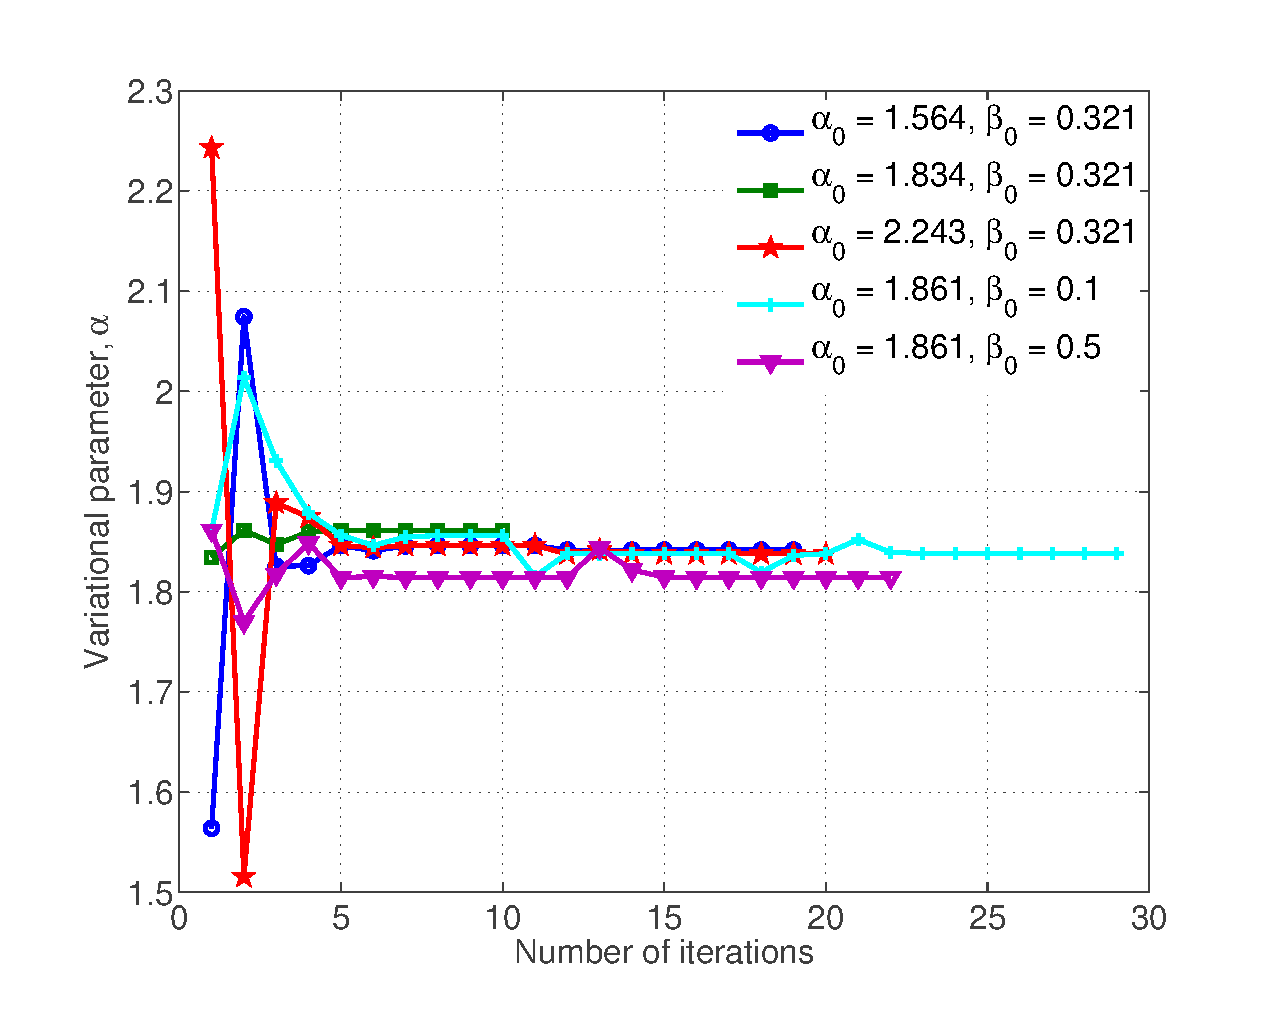
\includegraphics{experimentalData/parametricOptimization/alphaHeOptimizerFixedBeta}} \\
% % % % % % % % 			\resizebox{80mm}{!}{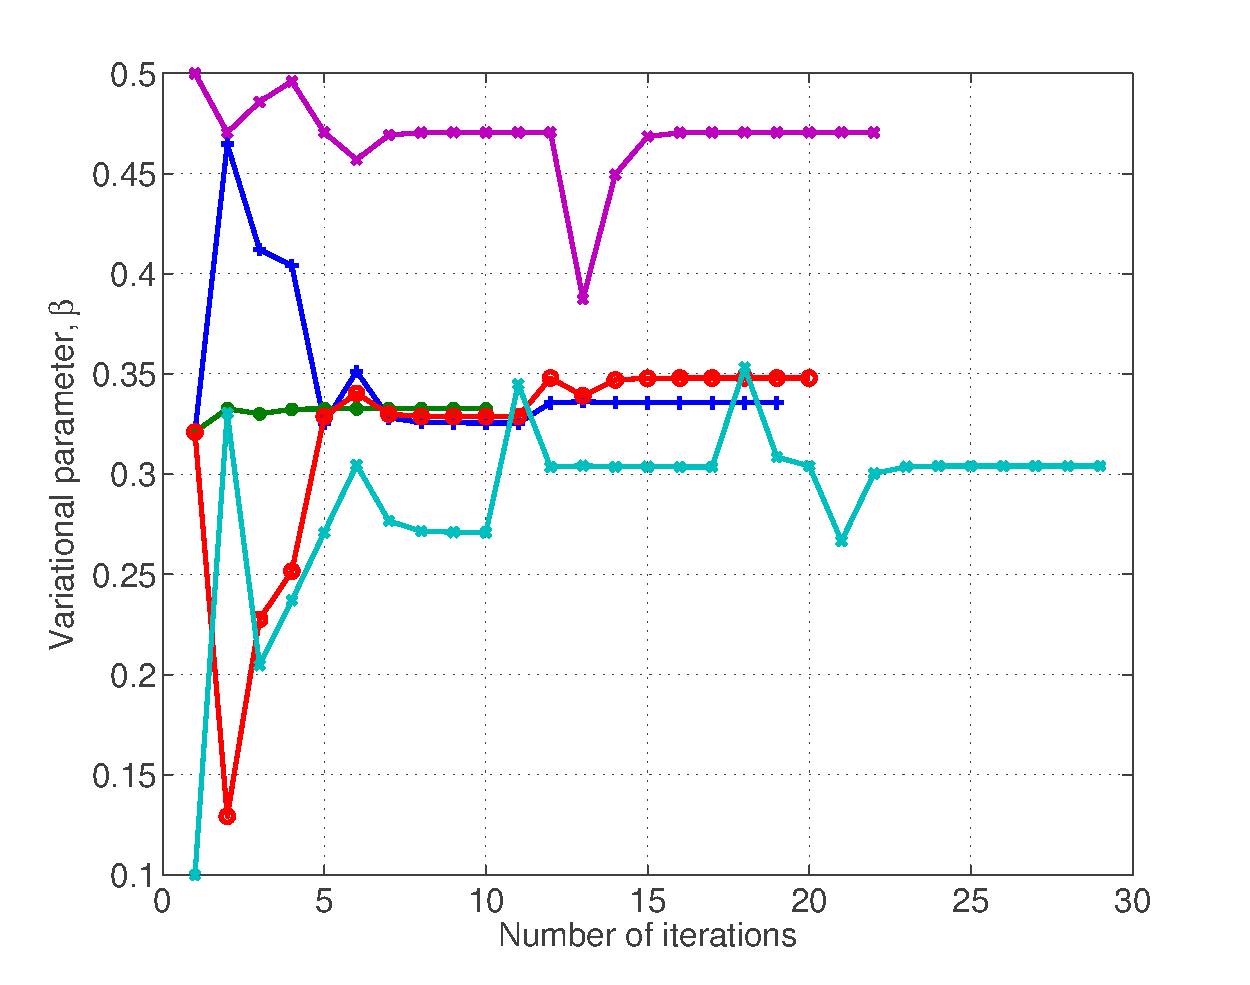
\includegraphics{experimentalData/parametricOptimization/BetaHeOptimizedFixedAlpha}} \\
% % % % % % % % 			 \resizebox{80mm}{!}{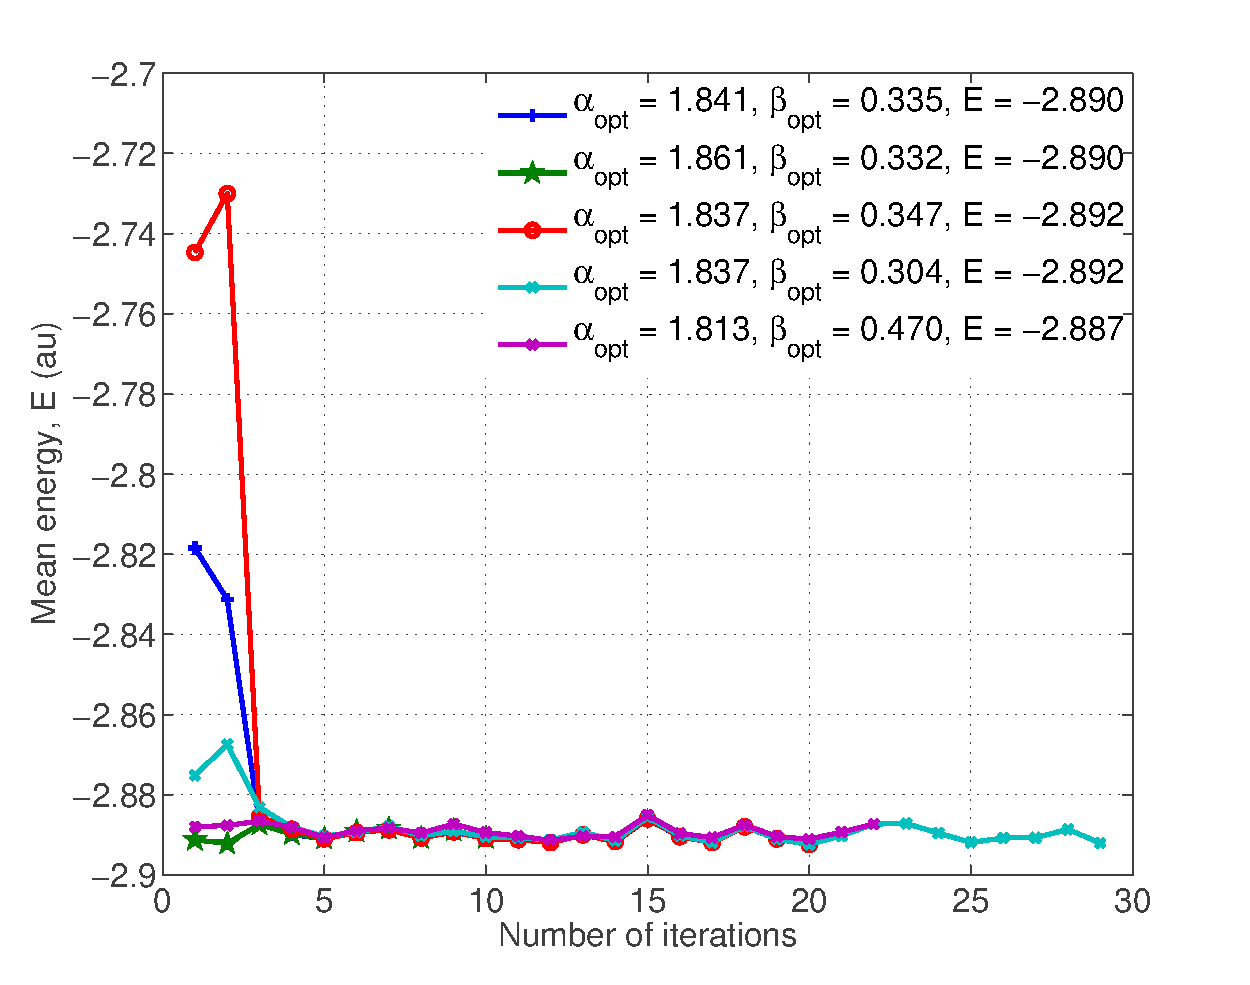
\includegraphics{experimentalData/parametricOptimization/energyHeAlphaBeta}}
% % % % % % % % 			 \end{tabular}
% % % % % % % %       \caption{Behaviour of the variational parameters $\alpha$ (top), $\beta$ (middle) and energy (bottom) for several start values of $\alpha$ and $\beta$ during the optimization of the trial wave function for He atom with quasi-Newton method. The experimental set up was: $dt = 0.01$, $1\times 10^7$ Monte Carlo cycles and 10 \% thermalization steps.}
% % % % % % % %       \label{optimizationHe}
% % % % % % % %     \end{center}
% % % % % % % %   \end{figure}
% % % % % % % % 	


% % % % % % % % % 
% % % % % % % % % 	\begin{figure}[!hbt]
% % % % % % % % %     \begin{center}
% % % % % % % % % 			 \begin{tabular}{cc}
% % % % % % % % % % % % %       \resizebox{75mm}{!}{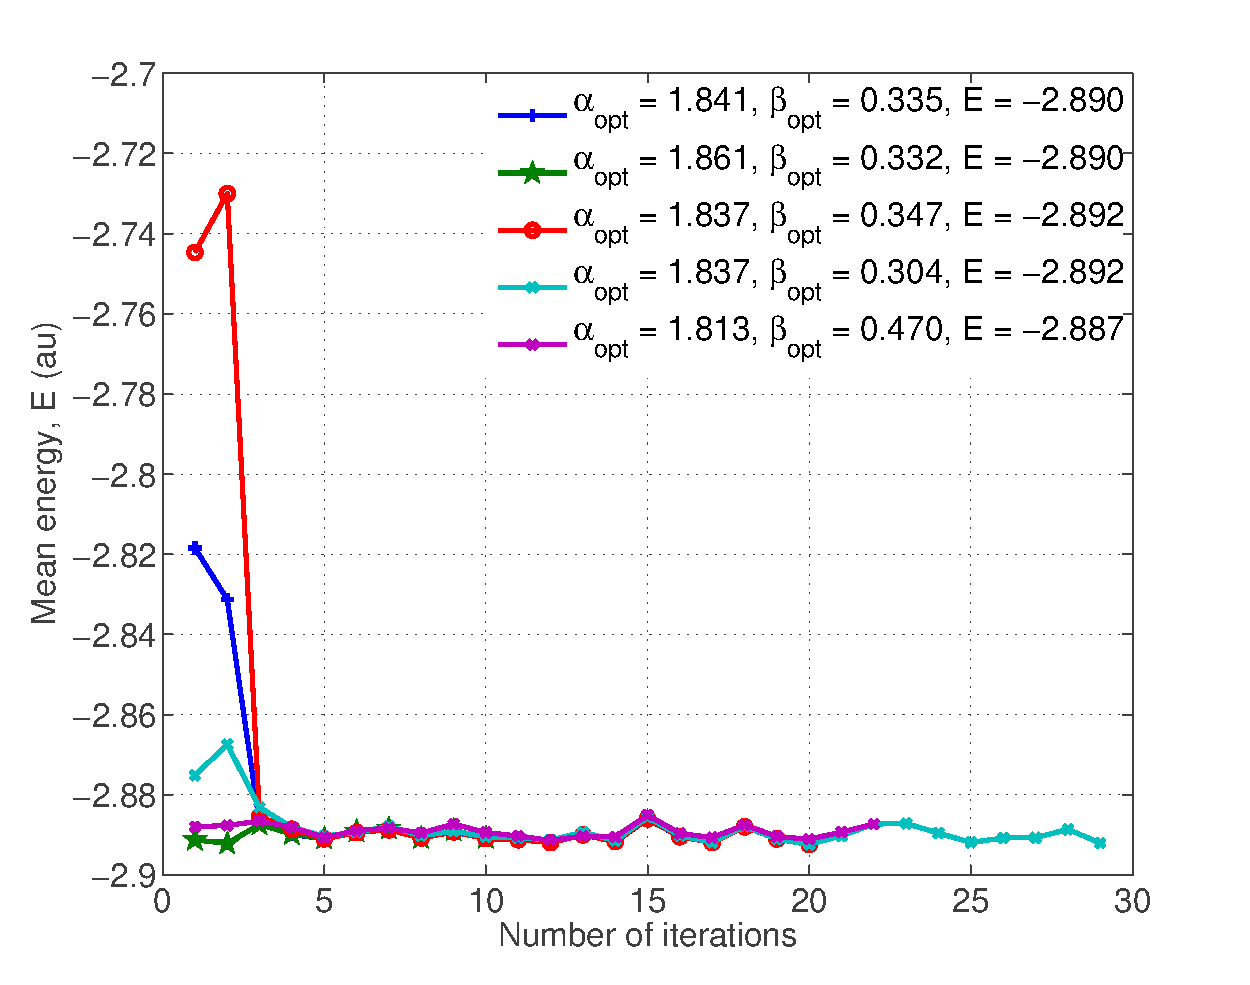
\includegraphics{experimentalData/parametricOptimization/energyHeAlphaBeta}} &
% % % % % % % % % 			\resizebox{80mm}{!}{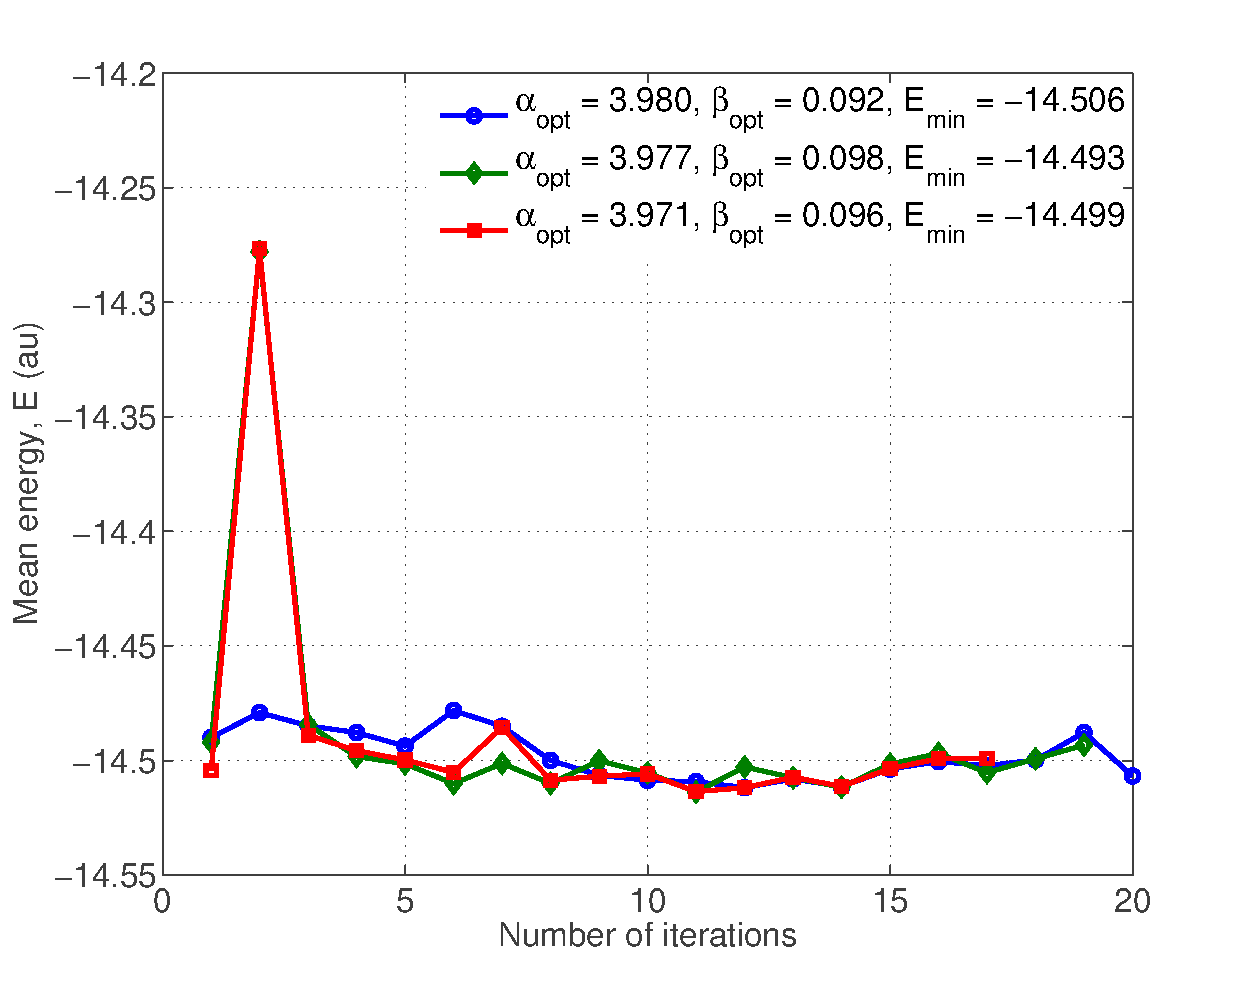
\includegraphics{experimentalData/parametricOptimization/energyBeAlphaBeta}}\\
% % % % % % % % % 			 \end{tabular}
% % % % % % % % %       \caption{}
% % % % % % % % %       \label{optimizationBe}
% % % % % % % % %     \end{center}
% % % % % % % % %   \end{figure}
% % % % % % % % % 	
% % % % % % % % % 	
% % % % % % % % % 	\begin{figure}[!hbt]
% % % % % % % % %     \begin{center}
% % % % % % % % % 			 \begin{tabular}{cc}
% % % % % % % % % % % % %       \resizebox{75mm}{!}{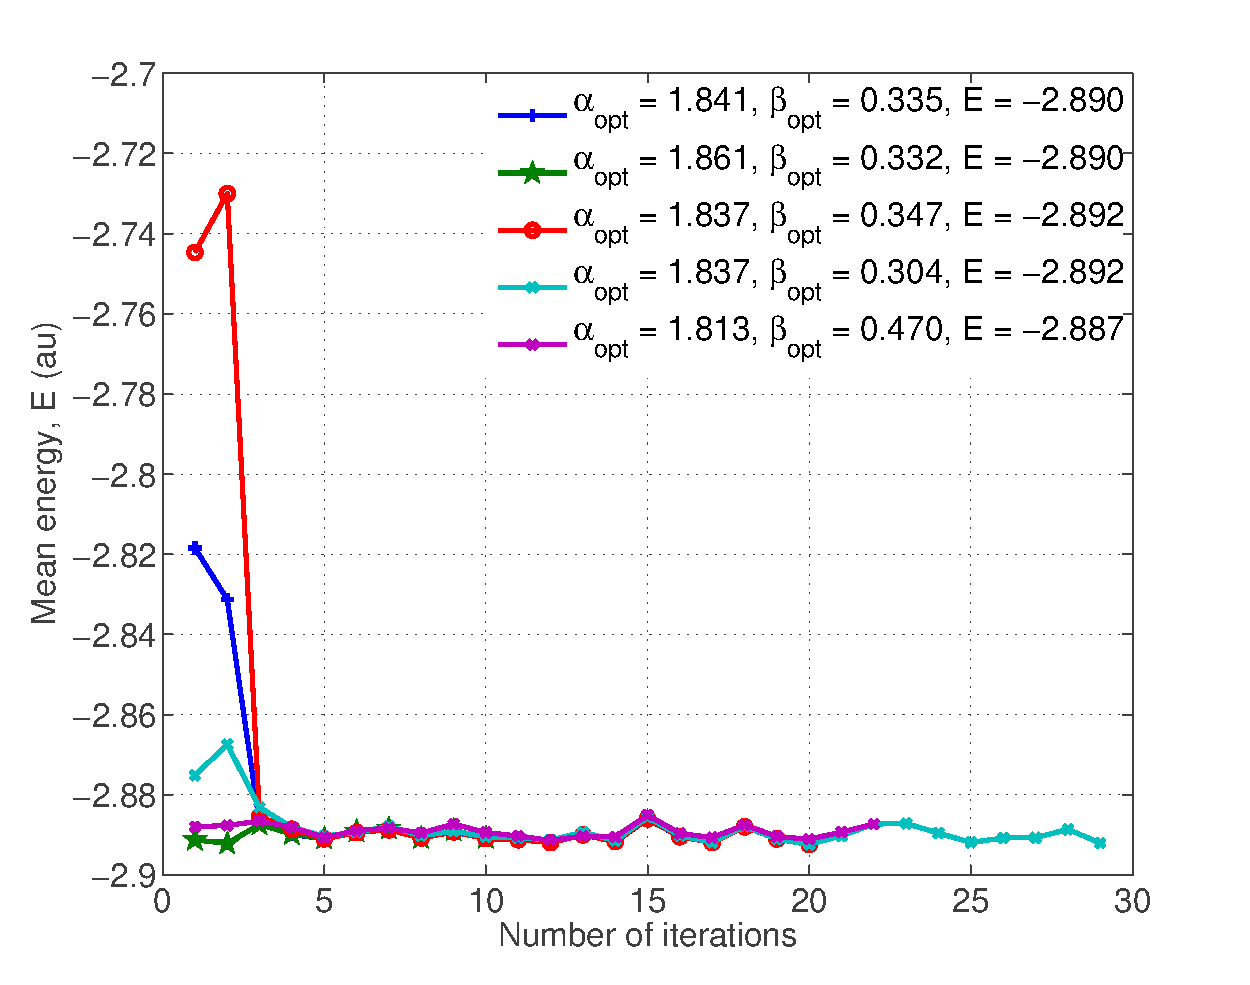
\includegraphics{experimentalData/parametricOptimization/energyHeAlphaBeta}} &
% % % % % % % % % 			\resizebox{80mm}{!}{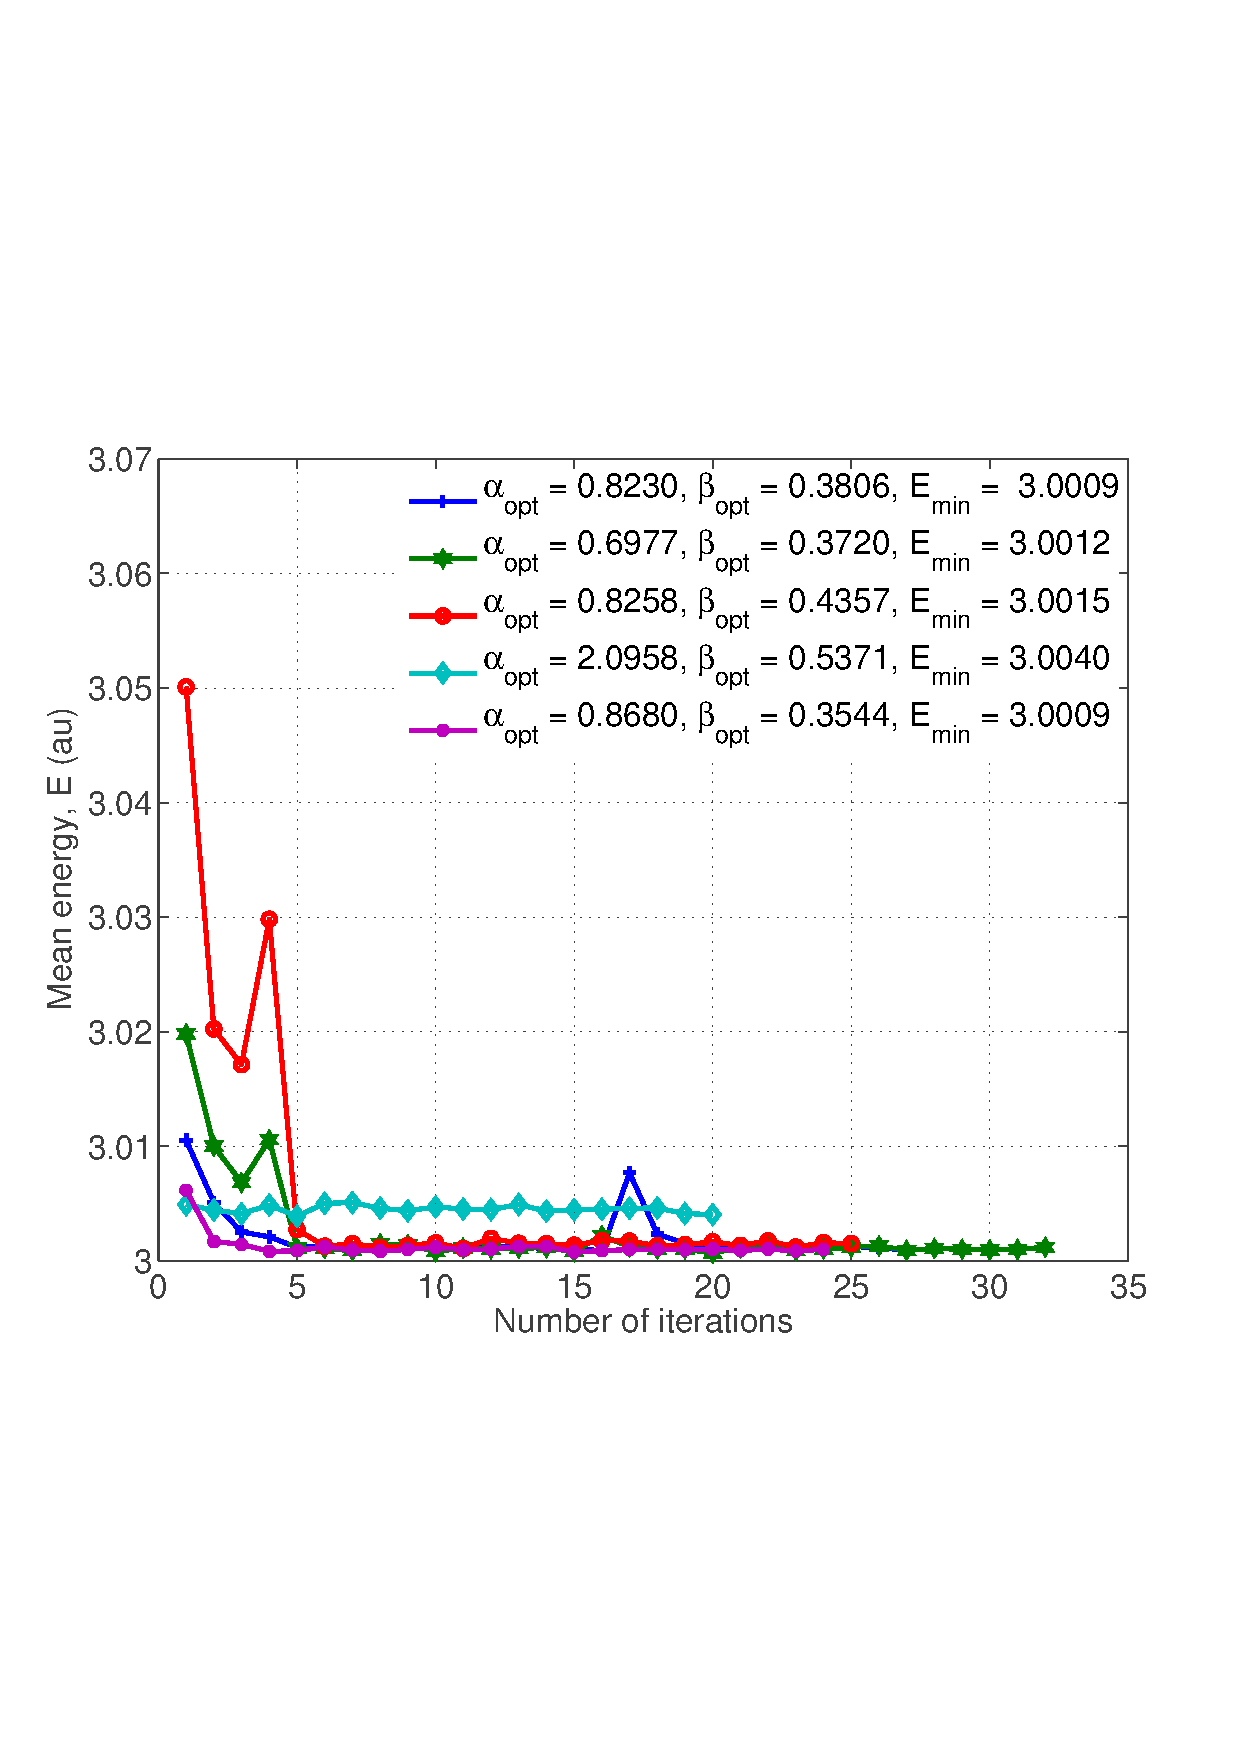
\includegraphics{experimentalData/parametricOptimization/energyAlphaBetaOptimizer2DQDot2e}}\\
% % % % % % % % % 			 \end{tabular}
% % % % % % % % %       %%%\caption{}
% % % % % % % % %       \label{optimizationBe}
% % % % % % % % %     \end{center}
% % % % % % % % %   \end{figure}

 
% % % % % % % % \begin{table}
% % % % % % % % \centering
% % % % % % % % \begin{tabular}{lccc}
% % % % % % % % \toprule[1pt]
% % % % % % % % \textbf{System} & $\alpha_{initial}$ & $\alpha_{optimum}$ & \textbf{error} \\
% % % % % % % % \midrule[1pt]
% % % % % % % % He  										&   		&   $1\times10^7$ & 10 \% \\
% % % % % % % % Be  										&   	&   $1\times10^7$ & 10 \%	\\
% % % % % % % % 2DHO2e ($\omega=1.0$)		&  &   $1\times10^7$ & 10 \%	\\
% % % % % % % % 2DHO6e ($\omega = 1.0$)	&  0.01  	& 	$1\times10^7$ & 10 \% \\
% % % % % % % % \bottomrule[1pt]
% % % % % % % % \end{tabular}\caption{Experimental set up to compute the dependence of the energy of the variational parameter $\alpha$ when no correlation is included. All the runs were carried out in serie.}
% % % % % % % % \label{expSetUpAlpha}
% % % % % % % % \end{table}
% % % % % % % % 

% % -Listar alpha y beta inciales, numero de iteraciones necesitadas y energias obtenidas en una tabla, con las respectivas enerigas finales para cada sistema estudiado. Comparar con resultados conocidos para sga (RUNE) y con el metodo grafico.


% % % First we studied the dependence of the optimal variational parameters and the minimum of the energy on the starting values 
% % % $\alpha_{0}$ and $\beta_0$. 
% % % % % The green line on the top and middle indicates that the number of iterations can be reduced considerably if we choose $\alpha_0$ and $\beta_0$ near the optimal values. \\
% % % \\
% % % % % In general, $\alpha$ converges more easily to the optimal value than $\beta$ and shows less oscillations. The convergence of $\beta$ depends greatly on its own start value and on the start value of $\alpha$. Moreover, different set of  variational parameters can give rise to the the same minimal energy.

